\PassOptionsToPackage{x11names}{xcolor}
\documentclass[3to2]{beamer}

\beamertemplatenavigationsymbolsempty


\usepackage{mathpartir}
\usepackage{bytefield}
\usepackage{tcolorbox}
\usetheme{jambro}
\usetikzlibrary{shapes}
\usepackage{catchfilebetweentags}
\makeatletter

\newrobustcmd*\OrigExecuteMetaData[2][\jobname]{%
\CatchFileBetweenTags\CatchFBT@tok{#1}{#2}%
\global\expandafter\CatchFBT@tok\expandafter{%
\expandafter}\the\CatchFBT@tok
}%\OrigExecuteMetaData

\newrobustcmd*\ChkExecuteMetaData[2][\jobname]{%
\CatchFileBetweenTags\CatchFBT@tok{#1}{#2}%
\edef\mytokens{\detokenize\expandafter{\the\CatchFBT@tok}}
\ifx\mytokens\empty\PackageError{catchfilebetweentags}{the tag #2 is not found\MessageBreak in file #1 \MessageBreak called from \jobname.tex}{use a different tag}\fi%
}%\ChkExecuteMetaData

\renewrobustcmd*\ExecuteMetaData[2][\jobname]{%
\ChkExecuteMetaData[#1]{#2}%
\OrigExecuteMetaData[#1]{#2}%
}

\makeatother

\usepackage{idris2}

\newcommand{\bobhead}{\includegraphics[scale=.2]{assets/bob.png}}
\newcommand{\mastodon}{\includegraphics[scale=.2]{assets/mastodon-logo-purple.png}}
\newcommand{\globe}{\includegraphics[scale=.1]{assets/globe.png}}

\newcommand{\smiley}{\includegraphics[scale=.025]{assets/robot-smiley.png}}
\newcommand{\sweaty}{\includegraphics[scale=.025]{assets/robot-sweaty.png}}
\newcommand{\stress}{\includegraphics[scale=.025]{assets/robot-stress.png}}
\newcommand{\clowny}{\includegraphics[scale=.025]{assets/robot-clowny.png}}
\newcommand{\scream}{\includegraphics[scale=.025]{assets/robot-scream.png}}

\newcommand{\source}{\includegraphics[scale=.1]{assets/tree.png}}
\newcommand{\target}{\includegraphics[scale=.1]{assets/wood.png}}
\newcommand{\beyond}{\includegraphics[scale=.1]{assets/flute.png}}

\newcommand{\saw}{\includegraphics[scale=.1]{assets/saw.png}}


\title{Correct by Construction Concurrent Programs \newline in Idris 2}
\author{Guillaume Allais}
\institute{University of Strathclyde \\ Glasgow, UK}
  \titlegraphic{BOB2025}
\date{March 14$^{th}$ 2025}

%% \AtBeginSection[]
%% {
%%     \begin{frame}
%%         \frametitle{Table of Contents}
%%         \tableofcontents[currentsection]
%%     \end{frame}
%% }

\usepackage{listings}
\lstset{language=Fortran,
  basicstyle=\ttfamily\bf,
  keywordstyle=\color{red},
}

%% Disable the >> ligature
\usepackage{microtype}
\DisableLigatures[>]{}

\begin{document}

\begin{frame}
  \maketitle
\begin{tikzpicture}[remember picture, overlay]
  \node[anchor=south east] at ($(current page.south east)+(0,.16)$){\bobhead};
\end{tikzpicture}
\end{frame}

{
\usebackgroundtemplate{%
  {\tikz{\node[opacity=0.2]{
    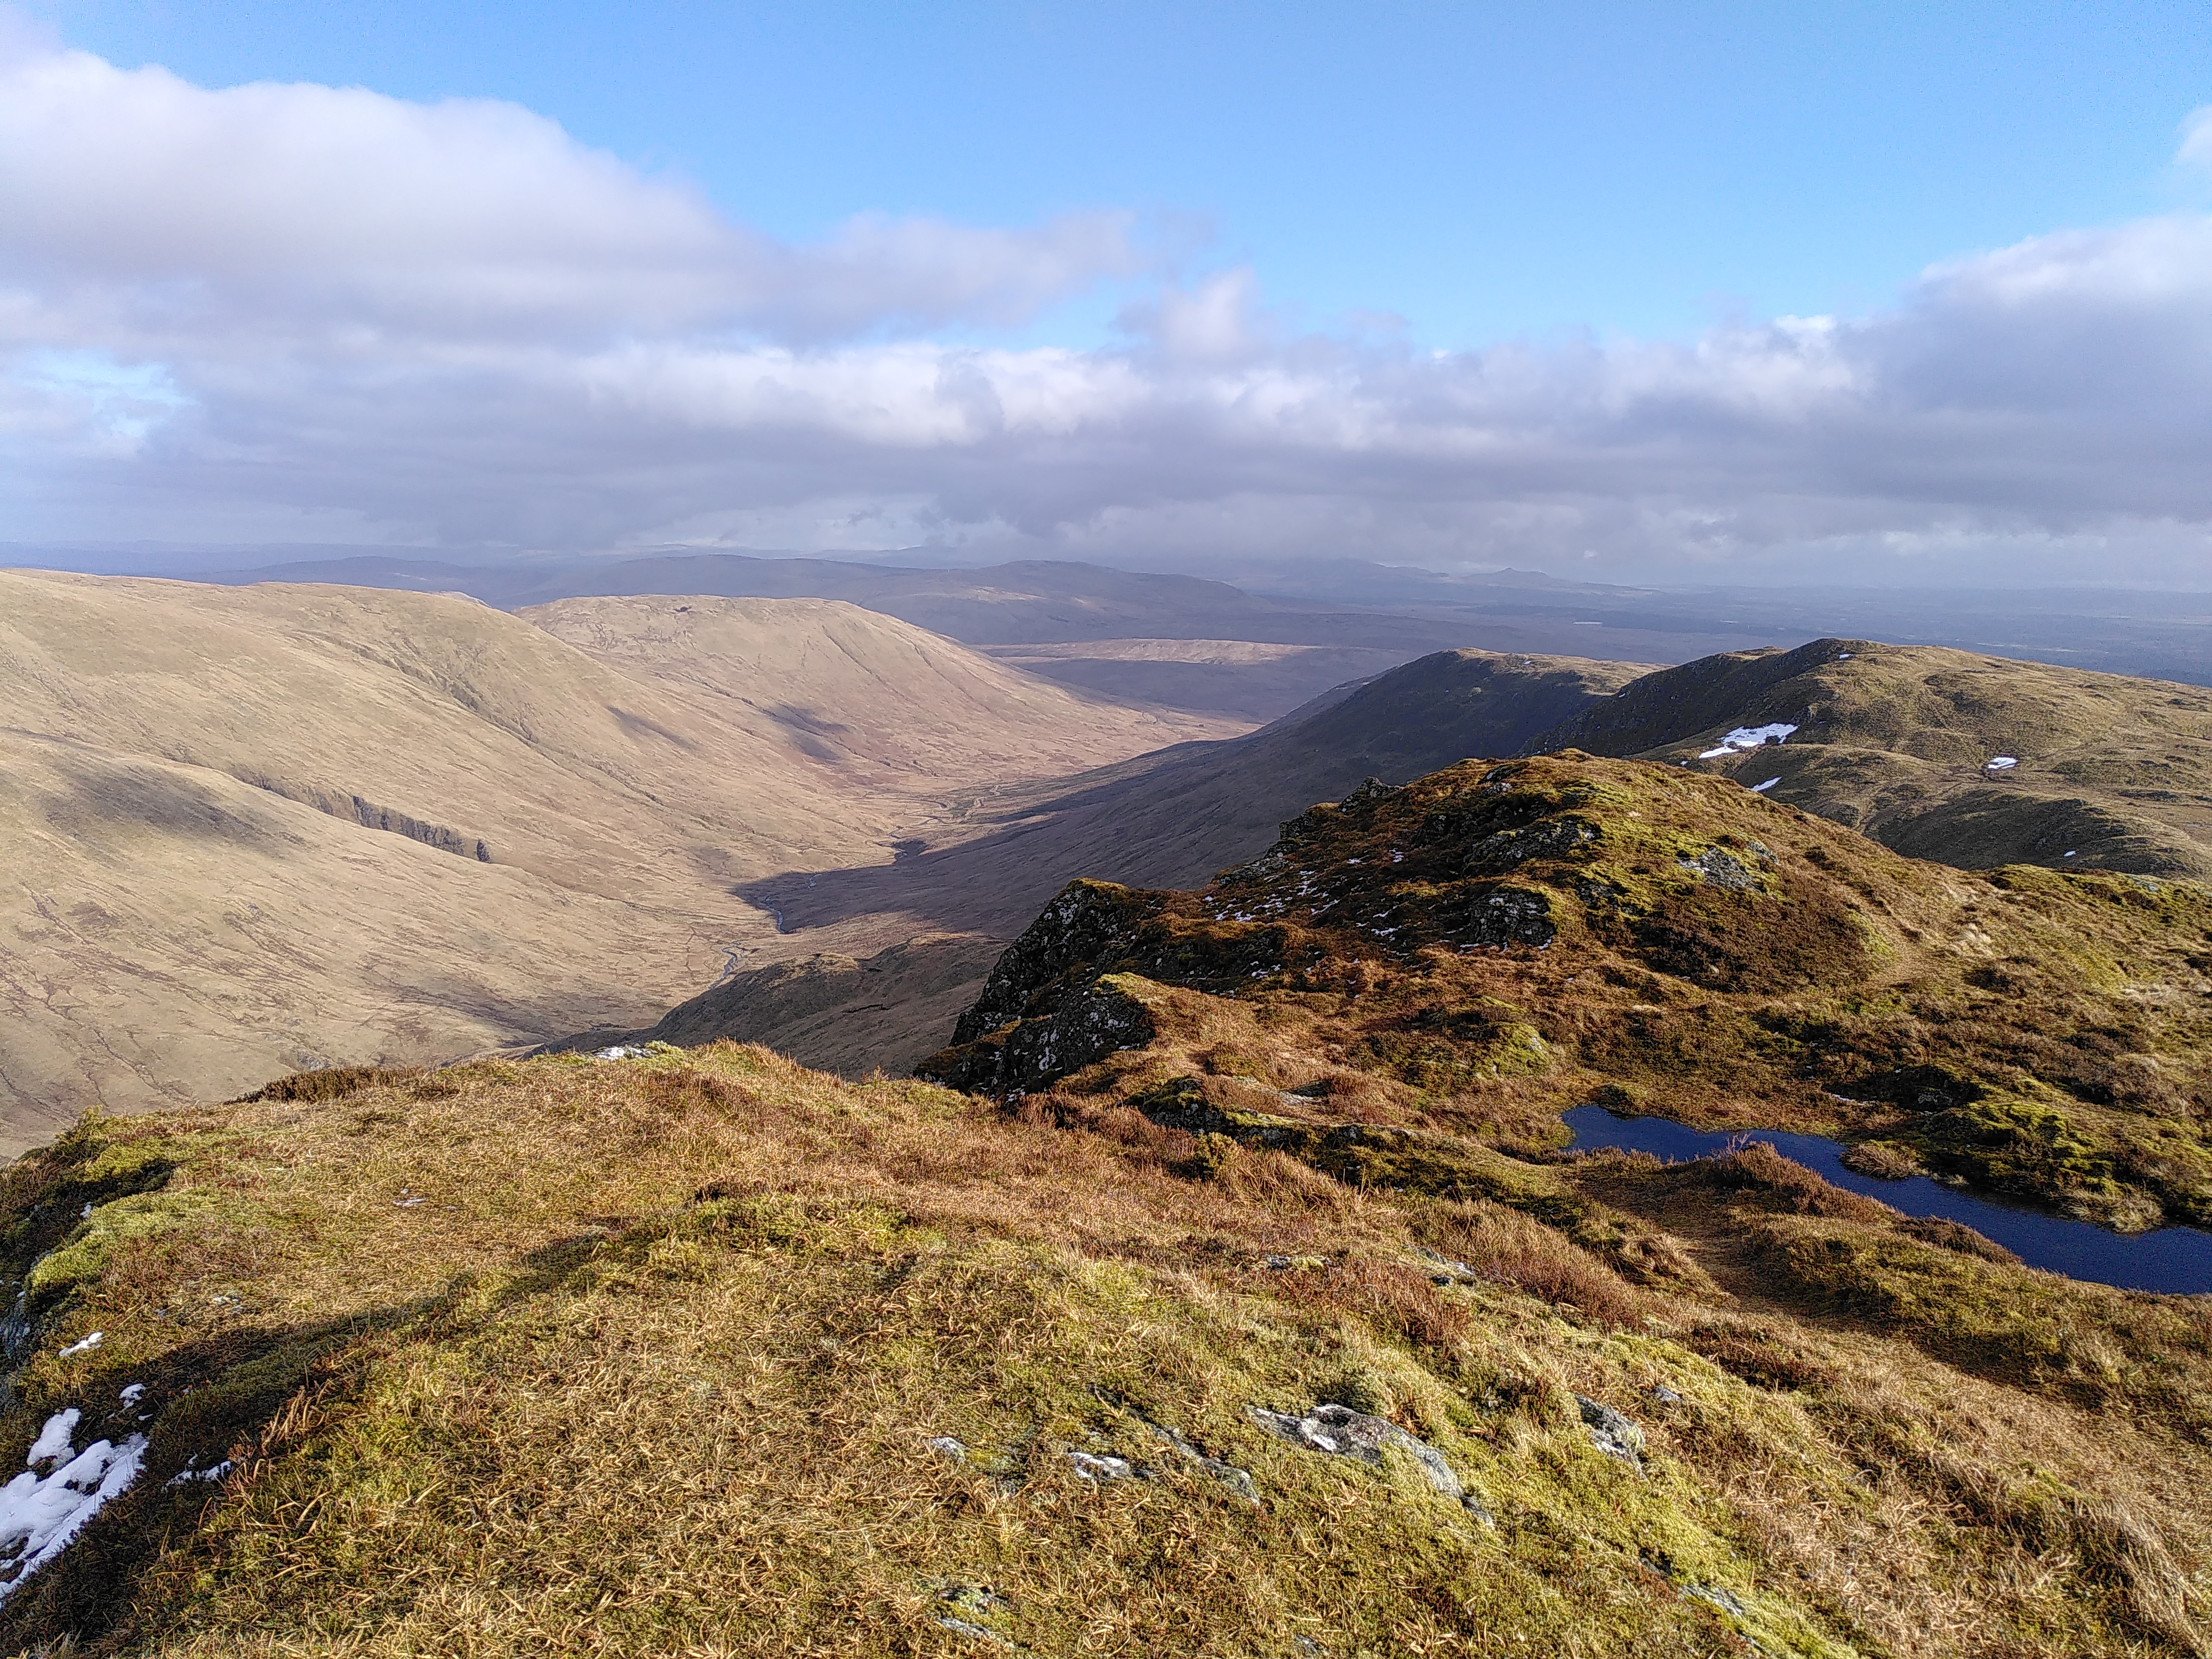
\includegraphics[width=\paperwidth]{assets/beinn_each.jpg}};}}}
\begin{frame}{About Me}
  Lecturer at the University of Strathclyde (Glasgow, Scotland)
  \vfill
  Interested in:
  \begin{itemize}
    \item Generic Programming and Proving
    \item Meta Programming and Proof Search
    \item Type-Directed Partial Evaluation
    \item Implementations of Type Theory
    \item Interactive Developer Tooling
  \end{itemize}
  \vfill
  Overarching Theme: Correctness by Construction
\end{frame}}

\section{Motivation}

\begin{frame}[fragile]{Sequential work}

One worker mapping the \saw{} transformation on a given array.

\bigskip

\begin{bytefield}[bitwidth=6mm, bitheight=8mm]{4}
 \\ \bitbox[]{1}{\alt<2>{\smiley}{}}
  & \bitbox[]{1}{\alt<3>{\smiley}{}}
  & \bitbox[]{1}{\alt<4>{\smiley}{}}
  & \bitbox[]{1}{\alt<5>{\smiley}{}}
  & \bitbox[]{1}{\alt<6>{\smiley}{}}
  & \bitbox[]{1}{\alt<7>{\smiley}{}}
  & \bitbox[]{1}{\alt<8>{\stress}{}}
  & \bitbox[]{1}{\alt<9>{\stress}{}}
  & \bitbox[]{1}{\alt<10>{\stress}{}}
  & \bitbox[]{1}{\alt<11>{\sweaty}{}}
  & \bitbox[]{1}{}
  & \bitbox[]{1}{}
  & \bitbox[]{1}{}
  & \bitbox[]{1}{}
  & \bitbox[]{1}{}
  & \bitbox[]{1}{}
  & \bitbox[]{1}{}
  & \bitbox[]{1}{}
  & \bitbox[]{1}{}
  & \bitbox[]{1}{}
  & \bitbox[]{1}{}

 \\ \bitbox[tbl]{1}{\alt<1>{\source}{\target}}
  & \bitbox[tb]{1}{\alt<1-2>{\source}{\target}}
  & \bitbox[tb]{1}{\alt<1-3>{\source}{\target}}
  & \bitbox[tb]{1}{\alt<1-4>{\source}{\target}}
  & \bitbox[tb]{1}{\alt<1-5>{\source}{\target}}
  & \bitbox[tb]{1}{\alt<1-6>{\source}{\target}}
  & \bitbox[tb]{1}{\alt<1-7>{\source}{\target}}
  & \bitbox[tb]{1}{\alt<1-8>{\source}{\target}}
  & \bitbox[tb]{1}{\alt<1-9>{\source}{\target}}
  & \bitbox[tb]{1}{\alt<1-10>{\source}{\target}}
  & \bitbox[tb]{1}{\source}
  & \bitbox[tb]{1}{\source}
  & \bitbox[tb]{1}{\source}
  & \bitbox[tb]{1}{\source}
  & \bitbox[tb]{1}{\source}
  & \bitbox[tb]{1}{\source}
  & \bitbox[tb]{1}{\source}
  & \bitbox[tbr]{1}{\source}
\end{bytefield}

\end{frame}

\begin{frame}[fragile]{Concurrent work}

Three concurrent workers mapping the \saw{} transformation on a shared array.

\bigskip

\begin{bytefield}[bitwidth=6mm, bitheight=8mm]{4}
 \\ \bitbox[]{1}{\alt<2>{\smiley}{}}
  & \bitbox[]{1}{\alt<3>{\smiley}{}}
  & \bitbox[]{1}{\alt<4>{\smiley}{}}
  & \bitbox[]{1}{\alt<5>{\smiley}{}}
  & \bitbox[]{1}{\alt<6>{\smiley}{}}
  & \bitbox[]{1}{\alt<7>{\smiley}{}}
  & \bitbox[]{1}{\alt<2>{\smiley}{\alt<8>{\scream}{}}}
  & \bitbox[]{1}{\alt<3>{\smiley}{}}
  & \bitbox[]{1}{\alt<4>{\smiley}{}}
  & \bitbox[]{1}{\alt<5>{\smiley}{}}
  & \bitbox[]{1}{\alt<6>{\smiley}{}}
  & \bitbox[]{1}{\alt<7>{\smiley}{}}
  & \bitbox[]{1}{\alt<2>{\smiley}{\alt<8>{\scream}{}}}
  & \bitbox[]{1}{\alt<3>{\smiley}{}}
  & \bitbox[]{1}{\alt<4>{\smiley}{}}
  & \bitbox[]{1}{\alt<5>{\smiley}{}}
  & \bitbox[]{1}{\alt<6>{\smiley}{}}
  & \bitbox[]{1}{\alt<7>{\smiley}{}}

 \\ \bitbox[tbl]{1}{\alt<1>{\source}{\target}}
  & \bitbox[tb]{1}{\alt<1-2>{\source}{\target}}
  & \bitbox[tb]{1}{\alt<1-3>{\source}{\target}}
  & \bitbox[tb]{1}{\alt<1-4>{\source}{\target}}
  & \bitbox[tb]{1}{\alt<1-5>{\source}{\target}}
  & \bitbox[tb]{1}{\alt<1-6>{\source}{\target}}

  & \bitbox[tb]{1}{\alt<1>{\source}{\alt<8>{\beyond}{\target}}}
  & \bitbox[tb]{1}{\alt<1-2>{\source}{\target}}
  & \bitbox[tb]{1}{\alt<1-3>{\source}{\target}}
  & \bitbox[tb]{1}{\alt<1-4>{\source}{\target}}
  & \bitbox[tb]{1}{\alt<1-5>{\source}{\target}}
  & \bitbox[tb]{1}{\alt<1-6>{\source}{\target}}

  & \bitbox[tb]{1}{\alt<1>{\source}{\alt<8>{\beyond}{\target}}}
  & \bitbox[tb]{1}{\alt<1-2>{\source}{\target}}
  & \bitbox[tb]{1}{\alt<1-3>{\source}{\target}}
  & \bitbox[tb]{1}{\alt<1-4>{\source}{\target}}
  & \bitbox[tb]{1}{\alt<1-5>{\source}{\target}}
  & \bitbox[tbr]{1}{\alt<1-6>{\source}{\target}}
\end{bytefield}

\end{frame}

\section{Hoare logic}

\newcommand{\addra}{\ensuremath{\ell_1}}
\newcommand{\addrb}{{\color{green} \ensuremath{\ell_2}}}

\begin{frame}{Hoare logic}

A logic for imperative programs.

A memory model.

\end{frame}

\begin{frame}{Assignment Axiom}
\begin{center}
    \huge
    \tikz[tstyle]{\node[nstyle](precondition){$\lbrace \ell \mapsto \text{\_} \rbrace$}}
    \quad
    \tikz[tstyle]{\node[nstyle](command){$\ell \mathbin{:=} 0$}}
    \quad
    \tikz[tstyle]{\node[nstyle](postcondition){$\lbrace \ell \mapsto 0 \rbrace$}}
\end{center}

\begin{tikzpicture}[tpstyle]
  \draw<2->[arrow,->] ([yshift=2pt]precondition.north) to[bend left] +(+.5,+2) node[anchor=south]
       {\hand Assuming that $\ell$ is a valid location};
  \draw<3->[arrow,->] ([yshift=2pt]command.north) to[bend left] +(1.6,+1) node[anchor=west]
       {\hand Assigning $0$ to $\ell$};
  \draw<4->[arrow,->] ([yshift=-2pt]postcondition.south) to[bend left] +(-1.6,-2) node[anchor=east]
       {\hand Ensures that $\ell$ points to $0$};
\end{tikzpicture}
\end{frame}


\begin{frame}{Sequential Execution Axiom}

{
  \huge
\begin{mathpar}
 \inferrule{
      \tikz[tstyle]{\node[nstyle](premise1){$\lbrace P \rbrace c_1 \lbrace Q \rbrace$}}
      \and \tikz[tstyle]{\node[nstyle](premise2){$\lbrace Q \rbrace c_2 \lbrace R \rbrace$}}
    }{\tikz[tstyle]{\node[nstyle](conclusion){$\lbrace P \rbrace c_1; c_2 \lbrace R \rbrace$}}}
\end{mathpar}}

\begin{tikzpicture}[tpstyle]
  \draw<2->[arrow,->] ([yshift=2pt]premise1.north) to[bend left] +(+0,+2) node[anchor=south]
       {\hand If $c_1$ takes us from $P$ to $Q$};
  \draw<3->[arrow,->] ([yshift=2pt]premise2.north) to[bend right] +(0,+1) node[anchor=south]
       {\hand And $c_2$ takes us from $Q$ to $R$};
  \draw<4->[arrow,->] ([yshift=-2pt]conclusion.south) to[bend left] +(+0,-1) node[anchor=north]
       {\hand Then the composition $c_1; c_2$ takes us from $P$ to $R$};
\end{tikzpicture}
\end{frame}

\begin{frame}{A proof: swap with no allocation}
  \Large
\[
\begin{array}{lr}
  & \uncover<2-9>{\lbrace \addra \mapsto a \wedge \addrb \mapsto b \rbrace}\\
  \addra \mathbin{:=} xor(\addra, \addrb);\\
  & \uncover<3->{\lbrace \addra \mapsto xor(a, b) \wedge \addrb \mapsto b \rbrace}\\
  \addrb \mathbin{:=} xor(\addra, \addrb);\\
  & \uncover<4->{
   \alt<4-5>
   {\lbrace \addra \mapsto xor(a, b)
        \wedge \addrb \mapsto \tikz[tstyle]{\node[nstyle](xorabb){$xor(xor(a,b),b)$}} \rbrace}
   {\lbrace \addra \mapsto xor(a, b) \wedge \addrb \mapsto a \rbrace}}\\
  \addra \mathbin{:=} xor(\addra, \addrb);\\
  & \uncover<7->{
   \alt<7-8>
   {\lbrace \addra \mapsto \tikz[tstyle]{\node[nstyle](xoraba){$xor(xor(a, b), a)$}}
        \wedge \addrb \mapsto a \rbrace}
   {\lbrace \addra \mapsto b \wedge \addrb \mapsto a \rbrace}}\\
 & \hphantom{\hphantom{\lbrace \addra \mapsto xor(a, b) \wedge \addrb \mapsto xor(xor(a,b),b) \rbrace}}
\end{array}
\]

\begin{tikzpicture}[tpstyle]
  \draw<5>[arrow,->] ([yshift=2pt]xorabb.south) to[bend left=10] +(-2.5,-1) node[anchor=north]
       {\hand $xor(xor(a,b),b)$ equals $a$};
  \draw<8>[arrow,->] ([yshift=-2pt]xoraba.south) to[bend left=10] +(-2.5,-1) node[anchor=north]
       {\hand $xor(xor(a,b),a)$ equals $b$};
\end{tikzpicture}
\end{frame}

\section{Separation logic}

\begin{frame}{$(\wedge)$ is the WRONG notion of ``and''}
\end{frame}

\section[Correct by Construction]{Correct by Construction Concurrent Programs}

\newcommand{\mathidris}[1]{{\bf{\mathtt{#1}}}}

\begin{frame}[fragile]{Old School Verification: Write, Test, Fix loop}
\begin{lstlisting}{Fortran}
  10 WRITE CODE
  20 DO FORMALISATION
  30 IF (CONTAINS BUG) THEN
  40   GOTO 10
  50 END IF
\end{lstlisting}
\end{frame}

\begin{frame}{Correct by Construction: Specify, Implement Correctly, Keep}
  Sometimes known as goal-driven development
  \vfill

  \begin{enumerate}
    \item Write a specification
    \item In a dialogue with the compiler interactively refine it
      \begin{itemize}
        \item Each step produces part of the program
        \item Some step introduce some further goals too
       \end{itemize}
    \item Keep refining until all goals are trivials
  \end{enumerate}
\end{frame}

\begin{frame}{In This Talk: Idris 2}
  \begin{itemize}
    \item<1-> Functional (lambdas, pure functions, inductive types)
      \only<1>{\ExecuteMetaData[Intro.idr.tex]{swap}}
    \item<2-> First class types (i.e. types are standard values)
      \only<2>{\ExecuteMetaData[Intro.idr.tex]{fileloc}}
    \item<3-> Resource-aware (separation of specification vs. runtime)
      \only<3-4>{\tikz[tstyle]{\node[nstyle](target){}}\ExecuteMetaData[Intro.idr.tex]{resource}}
    \item<5-> Strict (with explicit Laziness annotations)
    \item<6-> Compiled to ChezScheme (great target for a functional language)
    \item<7-> Self-hosted (reasonably fast!)
  \end{itemize}


\begin{tikzpicture}[tpstyle]
  \draw<4>[arrow,->] ([xshift=-8.2cm,yshift=-.9cm]target.south east) to[bend right] +(1.5,-1.2)
    node[anchor=west] {\hand Quantity $0$: erased during compilation};
\end{tikzpicture}
\end{frame}


\begin{frame}{In This Talk: Core Idea}
  Define a Domain Specific Language internalising
  Separation logic ideas

  \vfill
  \begin{itemize}
    \item<2-> Linearity (ab)used to ensure global uniqueness
    \item<3-> Ownership proofs instead of raw pointers
    \item<4-> Erasure to get rid of specification data (values showing up in $P$s, $Q$s, $R$s)
  \end{itemize}

\end{frame}

\begin{frame}{Ownership Type}


  $$\mathit{region}[\mathit{start}, \mathit{end}] \mapsto \mathit{vs}$$

  \ExecuteMetaData[Data/Buffer/Indexed.idr.tex]{owned}

\end{frame}

\newcommand{\listappend}{\mathop{+\!\!\!+}}

\begin{frame}{Read}
  $$\left\lbrace
    \uncover<2->{\begin{array}{cl}
      & \mathit{region}[\mathit{start}, \mathit{end}] \mapsto \mathit{vs}\\
      \uncover<3->{\sepconj & 0 \le \mathit{idx} < | \mathit{vs} |}
    \end{array}}
    \right\rbrace$$
  $$v = \mathidris{getBits8}(\mathit{idx});$$
  $$\left\lbrace
    \uncover<4->{\begin{array}{cl}
      & \mathit{region}[\mathit{start}, \mathit{end}] \mapsto \mathit{vs}\\
      \sepconj & v = \mathit{vs}[\mathit{idx}]
    \end{array}}
    \right\rbrace$$

  \uncover<5->{\ExecuteMetaData[Data/Buffer/Indexed.idr.tex]{read}}
\end{frame}

\begin{frame}{Write}
  $$\left\lbrace
    \uncover<2->{\begin{array}{cl}
      & \mathit{region}[\mathit{start}, \mathit{end}] \mapsto \mathit{vs}\\
      \uncover<3->{\sepconj & 0 \le \mathit{idx} < | \mathit{vs} |}
    \end{array}}
    \right\rbrace$$
  $$\mathidris{setBits8}(\mathit{idx}, \mathit{val});$$
  $$\left\lbrace
    \uncover<4->{\begin{array}{cl}
      & \mathit{region}[\mathit{start}, \mathit{end}] \mapsto \mathit{vs}[\mathit{idx} := \mathit{val}]\\
    \end{array}}
    \right\rbrace$$

  \uncover<5->{\ExecuteMetaData[Data/Buffer/Indexed.idr.tex]{write}}
\end{frame}

\begin{frame}{Split}
  $$\left\lbrace
    \uncover<2->{\begin{array}{cl}
      & \mathit{region}[\mathit{start}, \mathit{end}] \mapsto \mathit{vs} \listappend{} \mathit{ws}\\
      \uncover<3->{\sepconj & | \mathit{vs} | = \mathit{m}}
    \end{array}}
    \right\rbrace$$
  $$\mathidris{splitAt}(\mathit{m});$$
  $$\left\lbrace
    \uncover<4->{\begin{array}{cl}
        & \mathit{region}[\mathit{start}, \mathit{start} + \mathit{m}] \mapsto \mathit{vs}\\
        \sepconj & \mathit{region}[\mathit{start} + \mathit{m}, \mathit{end}] \mapsto \mathit{ws}
    \end{array}}
    \right\rbrace$$

    \uncover<5->{\ExecuteMetaData[Data/Buffer/Indexed.idr.tex]{split}}
\end{frame}

\begin{frame}{Combine}
  $$\left\lbrace
    \uncover<2->{\begin{array}{cl}
      & \mathit{region}[\mathit{start}, \mathit{middle}] \mapsto \mathit{vs}\\
      \sepconj & \mathit{region}[\mathit{middle}, \mathit{end}] \mapsto \mathit{ws}
    \end{array}}
    \right\rbrace$$
  $$\mathidris{combine}();$$
  $$\left\lbrace
    \uncover<3->{\begin{array}{cl}
      & \mathit{region}[\mathit{start}, \mathit{end}] \mapsto \mathit{vs} \mathop{+\!\!\!+} \mathit{ws}
    \end{array}}
    \right\rbrace$$

    \uncover<4->{\ExecuteMetaData[Data/Buffer/Indexed.idr.tex]{combine}}
\end{frame}


\begin{frame}{Map Type}
  \ExecuteMetaData[Data/Buffer/Indexed.idr.tex]{mapType}
\end{frame}

\begin{frame}{Sequential Map - Loop Type}
\hspace*{.1\textwidth}
\begin{bytefield}[bitwidth=6mm, bitheight=8mm]{4}
    \bitbox[]{1}{}
    \bitbox[]{1}{}
    \bitbox[]{1}{}
    \bitbox[]{1}{}
    \bitbox[]{1}{}
    \bitbox[]{1}{\smiley}
    \bitbox[]{1}{}
    \bitbox[]{1}{}
    \bitbox[]{1}{}
    \bitbox[]{1}{}
    \bitbox[]{1}{}
    \bitbox[]{1}{}
    \bitbox[]{1}{}
    \bitbox[]{1}{}
    \bitbox[]{1}{}
    \bitbox[]{1}{}
    \bitbox[]{1}{}
    \bitbox[]{1}{}
    \bitbox[]{1}{}
    \bitbox[]{1}{}
    \bitbox[]{1}{}

 \\ \bitbox[tbl]{1}{\tikz[tstyle]{\node[nstyle](target){\target}}}
    \bitbox[tb]{1}{\target}
    \bitbox[tb]{1}{\target}
    \bitbox[tb]{1}{\target}
    \bitbox[tb]{1}{\target}
    \bitbox[tb]{1}{\target}
    \bitbox[tb]{1}{\tikz[tstyle]{\node[nstyle](source){\source}}}
    \bitbox[tb]{1}{\source}
    \bitbox[tb]{1}{\source}
    \bitbox[tb]{1}{\source}
    \bitbox[tb]{1}{\source}
    \bitbox[tb]{1}{\source}
    \bitbox[tb]{1}{\source}
    \bitbox[tb]{1}{\source}
    \bitbox[tb]{1}{\source}
    \bitbox[tb]{1}{\source}
    \bitbox[tb]{1}{\source}
    \bitbox[tbr]{1}{\source}
\end{bytefield}

\vfill

\uncover<2->{
  \tikz[tstyle]{\node[nstyle](codepos){}}
  \ExecuteMetaData[Data/Buffer/Indexed.idr.tex]{loopty}
}

\begin{tikzpicture}[tpstyle]
  \node<3>[pencil,ultra thick,draw, minimum width=3.75cm, xshift=1.5cm, minimum height=.8cm, ellipse] (boxtarget) at (target) {};
  \node<4>[pencil,ultra thick,draw, minimum width=7.25cm, xshift=3.4cm, minimum height=.8cm, ellipse] (boxsource) at (source) {};
  \node<3>[pencil,ultra thick,draw, minimum width=3.5cm, xshift=8.5cm, yshift=-.65cm, minimum height=.8cm, ellipse] (codeboxtarget) at (codepos) {};
  \node<4>[pencil,ultra thick,draw, minimum width=1.55cm, xshift=11.9cm, yshift=-.65cm, minimum height=.8cm, ellipse] (codeboxsource) at (codepos) {};
\end{tikzpicture}

\end{frame}

\begin{frame}{Parallel Map}

{
    \uncover<2->{\ExecuteMetaData[Data/Buffer/Indexed.idr.tex]{halve}}
    \uncover<3->{\ExecuteMetaData[Data/Buffer/Indexed.idr.tex]{par1}}
    \uncover<4->{\ExecuteMetaData[Data/Buffer/Indexed.idr.tex]{parmaprec}}
}

\end{frame}

\begin{frame}{Parallel Reduce}
  Apply the same principles to get a parallel reduce

  Relying on monoid laws to prove correctness
\end{frame}


\begin{frame}{What's next?}
Separation logic has a lot more to offer!

  \begin{itemize}
    \item Partial ownership (shared reads, owned writes)
    \item Locks (non-deterministic access to shared resources)
    \item Ghost states (stateful specification data)
  \end{itemize}

\vfill

Use these building blocks!

  \begin{itemize}
    \item Richly typed parallel skeletons
    \item Reintroduce layers of abstractions (e.g. inductive types)
    \item Seamless programming over serialised data
    \item Concurrent programs
  \end{itemize}
\end{frame}

\begin{frame}{Happy to Chat!}
  \Large\centering
  \renewcommand\UrlFont{}
  \begin{tabular}{ll}
    \raisebox{-2pt}{\globe} &  \url{https://gallais.github.io} \\
    \raisebox{-4pt}{\mastodon} & \url{https://mamot.fr/@gallais}
  \end{tabular}
\end{frame}

\end{document}
